\receta{Molde Atún}

Rinde para 9 porciones.\\

\begin{ingredientes}
\item 312g Atun en aceite (drenado)
\item 1500g Papas
\item 125 ml Aceite de Oliva
\item 320g Cebolla de Huevo
\item 180g Pimentón
\item 150g Mayonesa
\item 4 Huevos
\item 100g Queso Parmesano
\item Pimiemta y sal al gusto
\end{ingredientes}
\preparacion

Papas peladas se cocinan en agua con sal hasta ablandar. Las papas cocidas se pasan por el presador para hacerlas puré. Al puré se le agrega: aceite de oliva para dar suavidad, sal y pimienta.

Se hiereven Los huevos se hasta que queden duros, partiendolos en rodajas y se reservan.

En una sartén, se ponen tiras de pimenton y cebolla a sofreir en aceite hasta dorar ligeramente. En una fuente, se mezcla la verdura sofritas, el atún escurrido y la mayoneza hasta obtener una mezcla homogenea. 

En un molde refractario plano se aplica una capa moderada de puré de papa, encima una capa de la mezcla de atún y verduras, encima una capa de rodajas de huevos y se termina con otra capa de puré de papa. Sobre la última capa de puré de papa se pone queso parmesano.\\

El molde se pone al horno a $170^{\circ}C$  a gratinar por 45 m inutos hasta obtener un color ligeramente dorado.\\

\vspace*{2cm}
\begin{center}
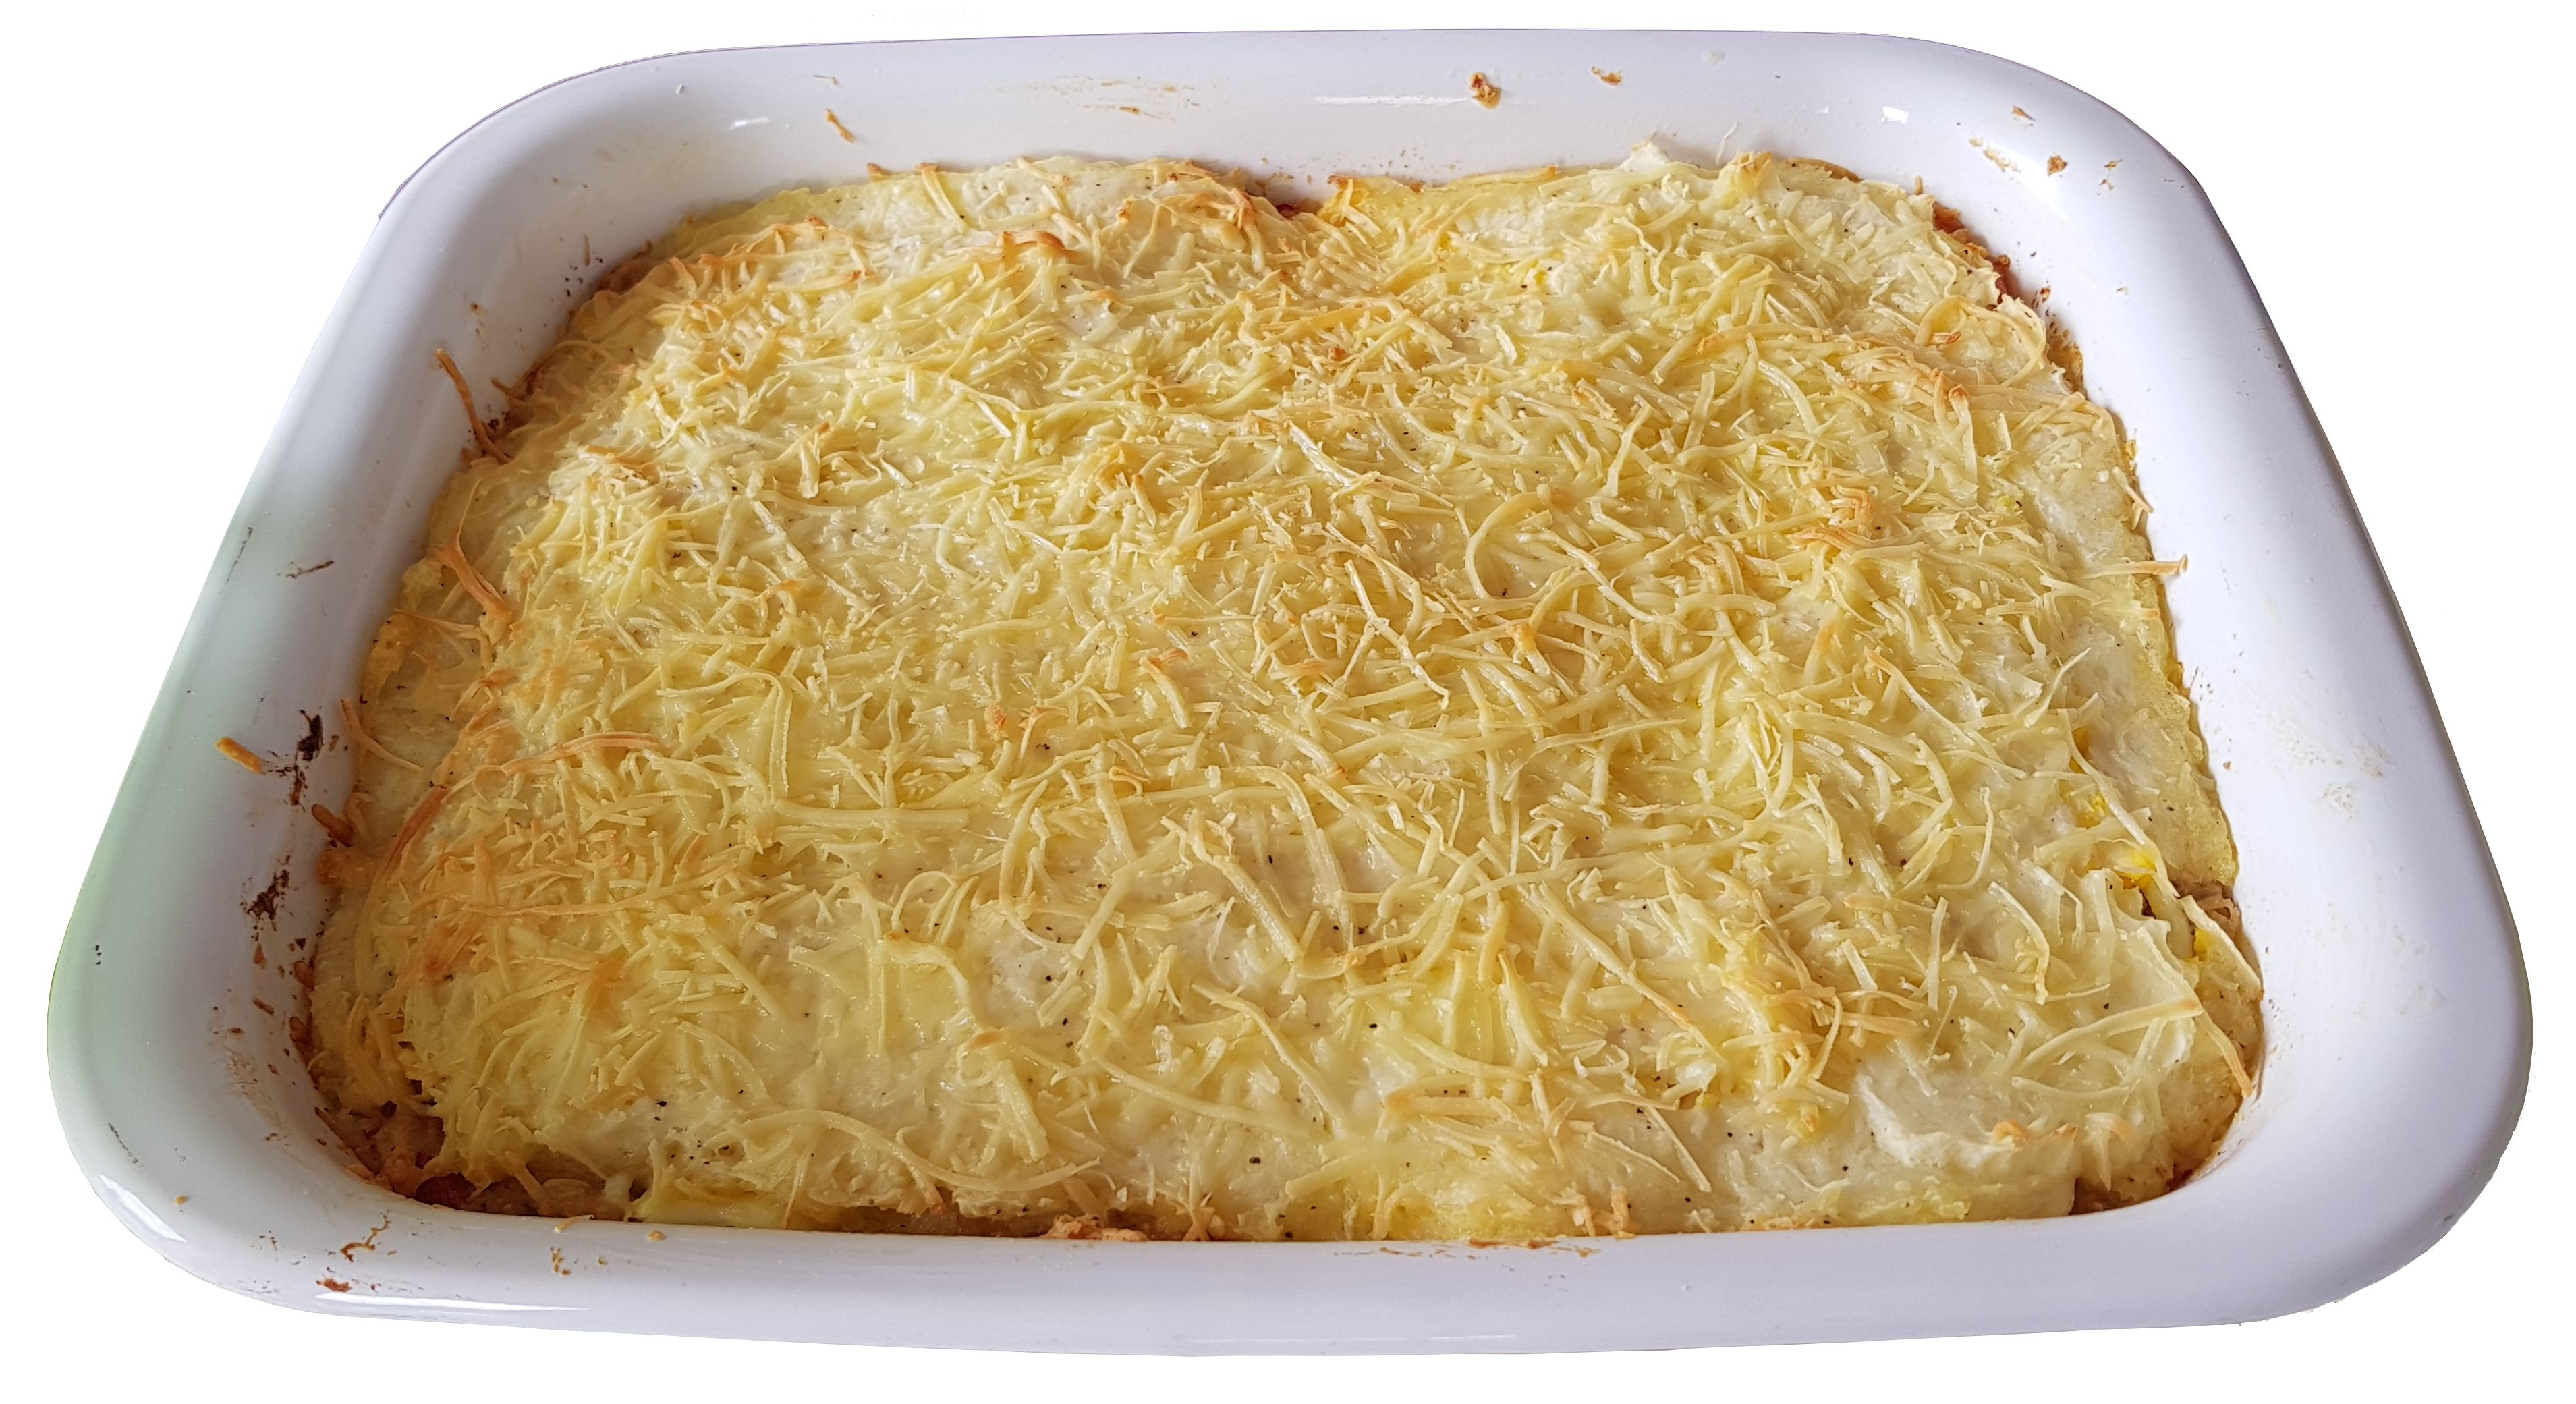
\includegraphics[width=0.8\textwidth]{fotos/molde_atun_2.jpeg}
\end{center}

\vspace*{2cm}
\begin{center}
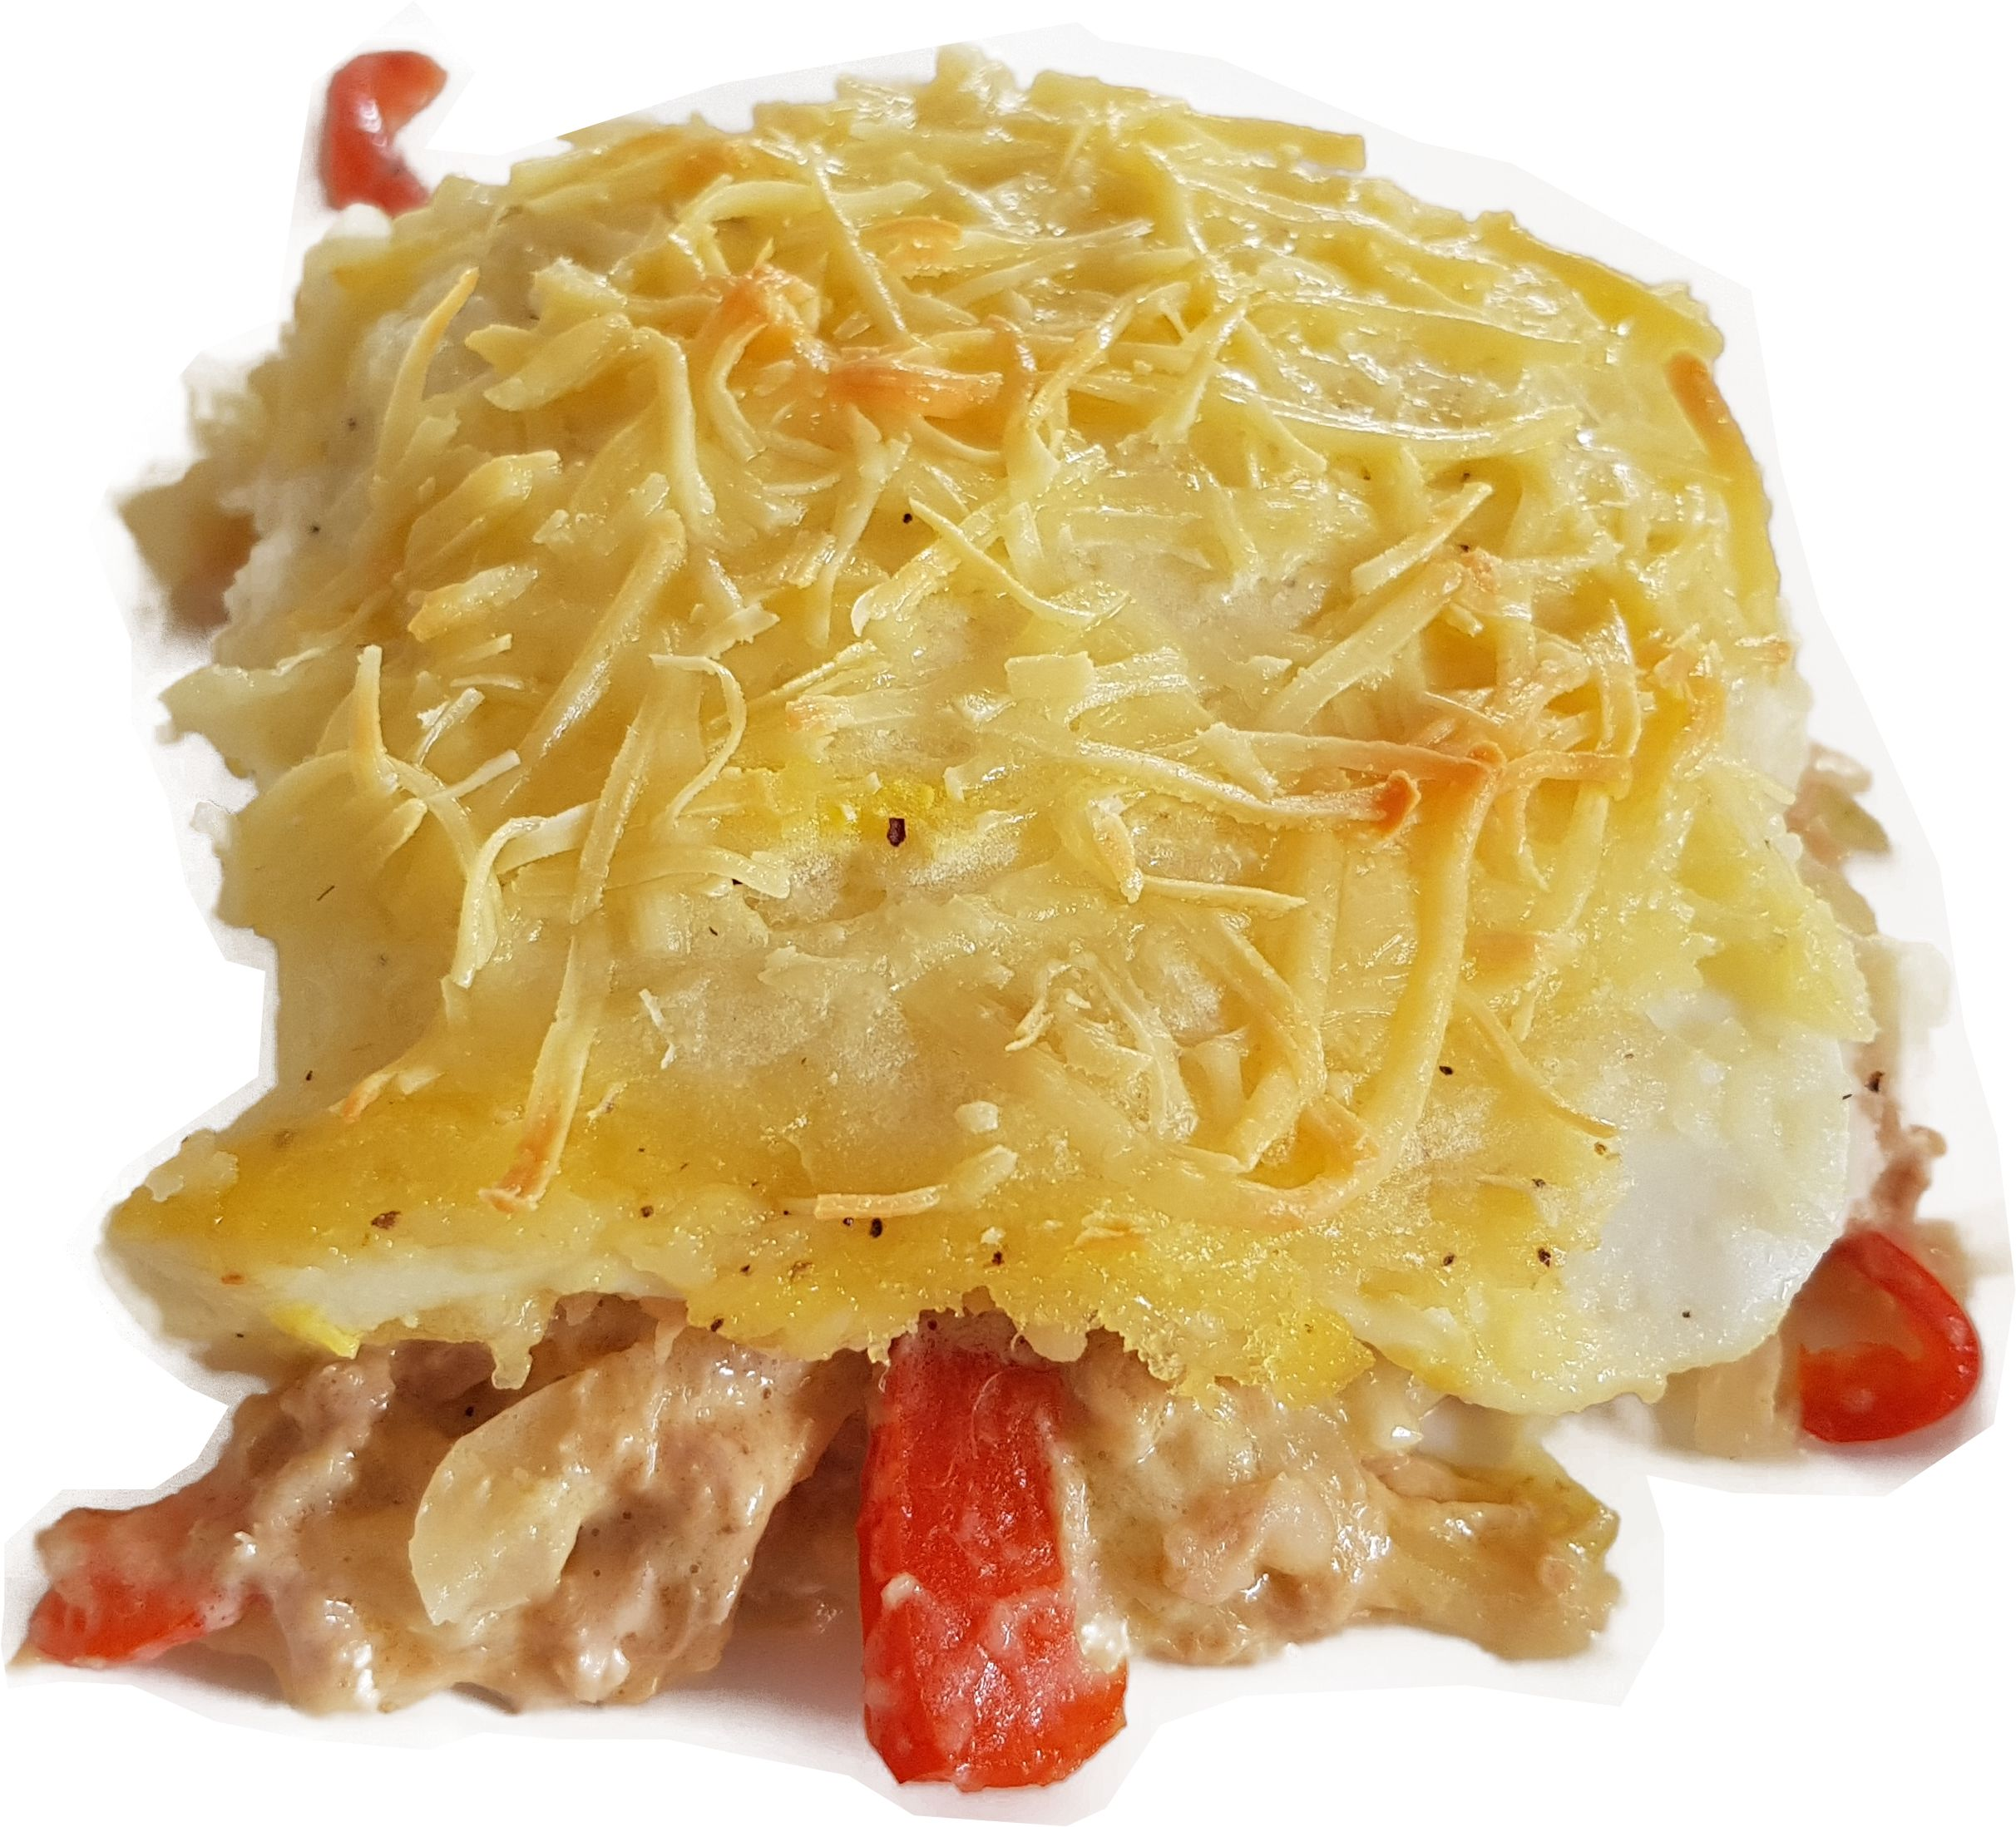
\includegraphics[width=0.8\textwidth]{fotos/molde_atun_1.jpeg}
\end{center}


